% Compilação (mesma configuração do vimtex): latexmk -pdf -lualatex -shell-escape -interaction=nonstopmode \
%           -synctex=1 -auxdir=.aux_files -bibtex main.tex

\documentclass[article,11pt,oneside,a4paper,brazil,section=TITLE]{abntex2}

\usepackage{iftex}
\ifLuaTeX
  \usepackage{fontspec}
  \setmainfont{Latin Modern Roman}
  \setsansfont{Latin Modern Sans}
  \setmonofont{Latin Modern Mono}
\else
  \usepackage[T1]{fontenc}
  \usepackage[utf8]{inputenc}
  \usepackage{lmodern}
\fi

\usepackage{graphicx}
\usepackage{booktabs}
\usepackage{tabularx}
\usepackage{microtype}
\usepackage[alf]{abntex2cite}

\graphicspath{{pictures/}}
\hypersetup{hidelinks}

\setlrmarginsandblock{2.2cm}{2.2cm}{*}
\setulmarginsandblock{2.2cm}{1.8cm}{*}
\checkandfixthelayout

\newcolumntype{Y}{>{\raggedright\arraybackslash}X}

\titulo{Automação com IA e Segurança: triagem de cadastros com n8n e LLM}
\autor{Gabriel Salmoria}

\begin{document}
\textual

\begin{center}
  {\small
    UNIVERSIDADE FEDERAL DE SANTA CATARINA\\
    Departamento de Informática e Estatística\\
    INE5448 --- Tópicos Especiais em Aplicações Tecnológicas I\par}
  \vspace{1.2em}
  {\bfseries\large Automação com IA e Segurança:\\
   triagem de cadastros com n8n e LLM\par}
  \vspace{0.8em}
  {Gabriel Salmoria \quad --- \quad \today\par}
\end{center}
\vspace{1em}

% =====================================================================
\section{O problema e o fluxo}

Um formulário público de filmes favoritos (ideia é replicar um forms publico, que é passado como TCC e afnis) com caixas de texto livre que alguém precisa ler, padronizar e repassar internamente. O fluxo construído automatiza esse trabalho, apenas recebe a submissão, valida os campos, usa uma LLM para reestruturar uma versão organizada das informações e envia o resultado por e-mail para um endereço interno (equivalente de salvar num sistema ou planilha, apenas com menos problemas de conexão de OAuth, pra simplificar a demo).

O formulario coleta nome, e-mail, idade e um texto livre sobre o filme favorito. Ele é aberto, sem autenticação, afinal a intenção e receber cadastros de qualquer pessoa. Por motivos de demonstracao, há uma regra adicional, sendo q cadastros de menores de idade não geram e-mail (ex: Tratamento diferente à menores devido à uso de dados), apenas registro em banco internamente.

O video de explicação da arquitetura e do fluxo segue em: https://youtu.be/j666yIm5e1E

\subsection{Arquitetura}

O fluxo tem oito \emph{nodes} principais e dois subnodes, acima do mínimo de
quatro exigido. A Figura~\ref{fig:fluxo} mostra o editor do n8n.

\begin{itemize}\setlength{\itemsep}{1pt}
  \item \textbf{On form submission} (\emph{Form Trigger}): ponto de entrada do forms.

  \item \textbf{Valida e sanitiza entrada} (\emph{Code}): valida os campos e detecta tentativas de \emph{prompt injection}.

  \item \textbf{entrada suspeita?} (\emph{IF}): separa as submissões aprovadas das bloqueadas.

  \item \textbf{registra tentativa bloqueada} (\emph{Data Table}): grava a submissão rejeitada com o motivo e encerra o fluxo.

  \item \textbf{adiciona os dados do usuario no BD} (\emph{Data Table}): grava o cadastro aprovado.

  \item \textbf{IA} (\emph{AI Agent}): redige o texto do e-mail. Usa o subnode \textbf{Groq} (modelo \texttt{openai/gpt-oss-20b}) e um \textbf{Structured Output Parser}, que força a saída no formato \texttt{\{title, text\}}. \item \textbf{usuario maior de idade?} (\emph{IF}): compara a idade com 18.

  \item \textbf{Envia email interno} (\emph{Gmail}) e \textbf{nao envia o email} (\emph{Data Table}): saídas dos ramos adulto e menor.
\end{itemize}

\begin{figure}[htb]
  \centering
  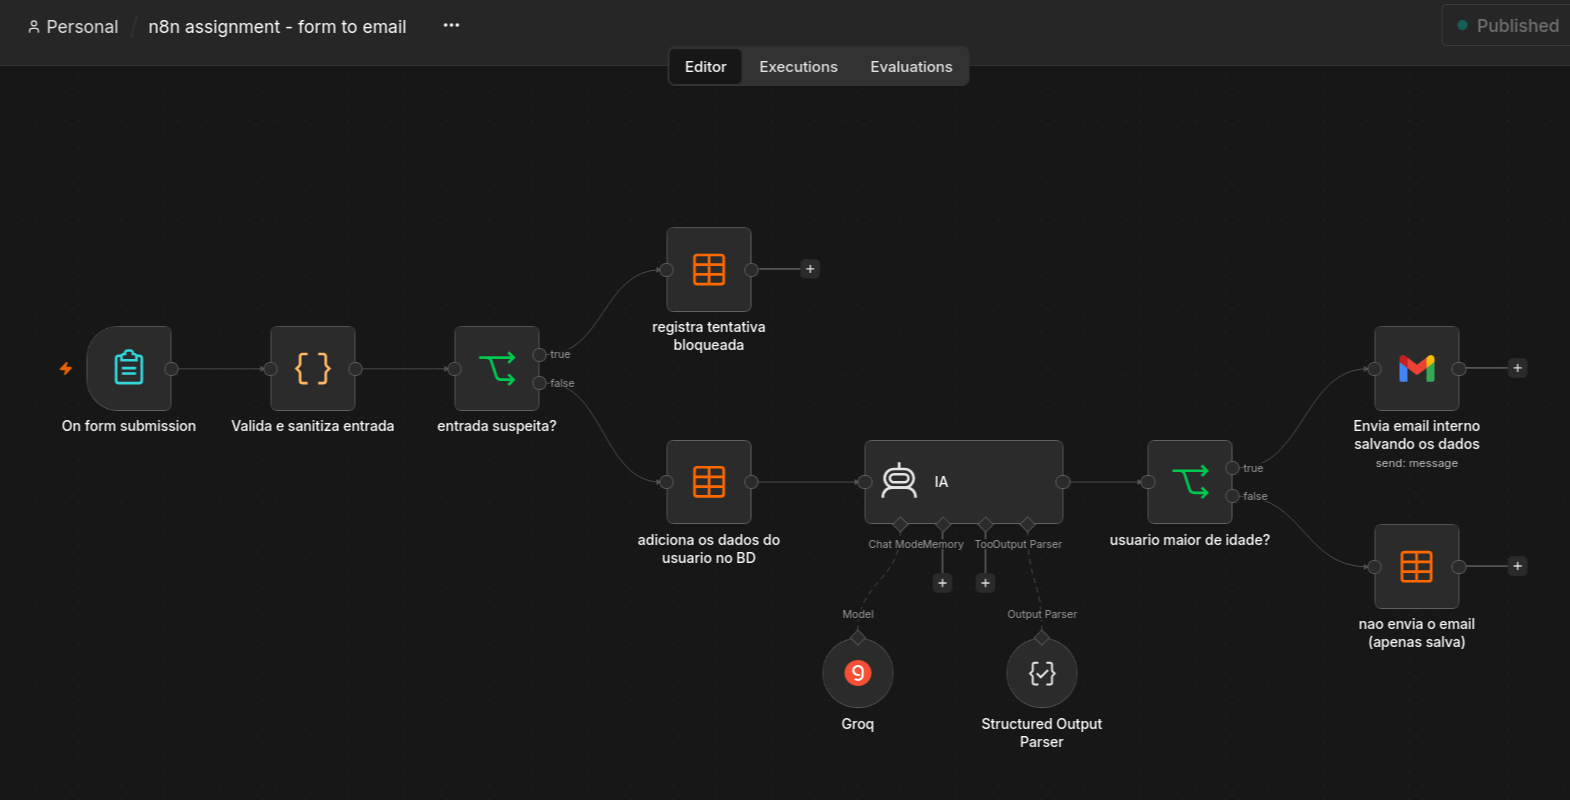
\includegraphics[width=\textwidth]{fluxo-n8n.png}
  \caption{Fluxo no editor do n8n.}
  \label{fig:fluxo}
\end{figure}

% =====================================================================
\section{Análise de segurança}

\subsection{Gestão de chaves de API}

As credenciais do Groq e do Gmail ficam no sistema de \emph{Credentials} do n8n e não em parametros de \emph{node}. No arquivo exportado aparece apenas a referencia \texttt{\{"id": ..., "name": "Groq account"\}}, sem nenhuma API key ou credencial vazada. Isso foi conferido com uma varredura do JSON procurando por prefixos de chave (\texttt{gsk\_}, \texttt{sk-}), \emph{tokens bearer} e campos de senha, sem resultados.

Não a rotação (ou troca) automatica de chaves, a troca seria manual, pelo console do Groq e atualizando o n8n. Se a chave do Groq vazasse o impacto seria consumo de cota e custo, já que ela da acesso apenas a API de inferencia. O caso do Gmail é mais grave, por que é um OAuth2 com permissao de envio, mas esse \emph{token} fica cifrado no n8n e não é exportado. Como medida preventiva vale definir limite de gasto na conta do provedor. Portanto não usar as credenciais no proprio fluxo, como usado, é essencial para manter a seguranca da aplicacao.

\subsection{Autenticação e autorização}

O acesso ao editor do n8n é protegido por conta e senha da plataforma, via cloud apenas com as credenciais do operador (eu).

O \emph{trigger} do formulário não tem autenticação, e isso é uma decisão de projeto com intuito de replicar um google forms generico, exigir credencial num formulário público de cadastro acabaria com a função dele. Como qualquer pessoa com a URL pode acionar o fluxo, o controle não fica na entrada, e sim na validação em código logo depois do \emph{trigger}. O risco que sobra é abuso por volume, enchendo as tabelas e consumindo a cota do Groq. A mitigação proposta é limitacao de taxa e \emph{CAPTCHA} no formulário ou possiveis eventuais soluções de \emph{rate-limiting}.

\subsection{Proteção de dados}

O formulário coleta dados pessoais: nome, email e idade. Nos testes foram usados dados fictícios.

Toda entrada passa pelo \emph{node} \texttt{Valida e sanitiza entrada} antes de qualquer uso. A higienização remove caracteres especiais, colapsa quebras de linha, apaga os caracteres \texttt{<} e \texttt{>} e trunca cada campo (80, 120 e 800 caracteres). A validação rejeita nome vazio, e-mail malformado e idade que não seja inteiro entre 0 e 120. Essa parte é necessaria pq nenhum campo do \emph{Form Trigger} é obrigatório, entao uma submissão vazia chegaria aos \emph{nodes} seguintes sem tratamento. Os \emph{nodes} seguintes usam apenas os campos já higienizados. Duas limitações sobram. A primeira é que os dados passam por terceiros: o n8n Cloud executa o fluxo e o Groq recebe o conteúdo do formulário, o que num caso real deveria estar num self hosting e IAs proprias. A segunda é a verificacao de idade acontecendo depois da LLM, então os dados de um menor são gravados na primeira tabela e enviados ao Groq antes de a condição ser avaliada. O controle atual evita o e-mail, mas não o processamento. Considerando o tratamento mais restritivo que a LGPD~\cite{lgpd} dá aos dados de crianças e adolescentes, mover a verificação de idade para antes do \emph{node} de IA seria a melhoria mais relevante do fluxo (o que, num caso real, não causaria problemas, devido a rodar a IA localmente).

\subsection{Segurança do ambiente}

A execução usa o n8n Cloud, e não uma instância local. como o acesso é feito só por HTTPS com certificado gerenciado e as atualizações da plataforma são aplicadas pelo fornecedor, elimina-se os problemas comuns de uma instância em self hosted exposta sem TLS ou desatualizada. Em compensação, os dados são processados na infraestrutura de um terceiro e não a controle rigido sobre regras de rede ou tratamento de dados internos. Para um exercício com dados inventados, a troca compensa.

\subsection{Riscos do LLM}

O campo de texto livre é enviado a um \emph{prompt} cujo resultado vira assunto e corpo de um e-mail. É o cenário clássico de \emph{prompt injection}, apontado como principal risco de aplicações integradas a LLMs~\cite{owasp,greshake2023}. A defesa é feita em:

A primeira é a detecção em código, antes do LLM. O \emph{node} de validação aplica dez expressões regulares sobre o texto original, procurando sobrescrita de instruções (\emph{``ignore as instruções anteriores''}), redefinição de papel, turnos falsos de conversa (\texttt{system:}), tentativa de forjar o delimitador, exfiltração do \emph{prompt} e redirecionamento do e-mail. A detecção roda antes da higienização, porque a limpeza apagaria as evidências. Havendo indício, a submissão é marcada como suspeita, gravada na tabela \texttt{blocked requests} junto com o motivo, e o fluxo termina sem chamar o LLM.

A segunda é a separação entre instrução e dado no \emph{prompt}. O conteúdo do usuário fica dentro de \texttt{<dados\_usuario>}, com instrução explícita de tratar aquilo como texto e nunca como comando. A remoção de \texttt{<} e \texttt{>} na higienização é o que sustenta essa camada, porque impede o usuário de fechar o delimitador antes da hora.

A terceira é estrutural, e é a mais confiável das três: o \emph{Structured Output Parser} obriga a saída a ter o formato \texttt{\{title, text\}} e o destinatário no \emph{node} do Gmail é fixo. Uma injeção, mesmo que bem sucedida, não consegue redirecionar a mensagem nem produzir saída de formato genérico ou usável por um atacante. O pior caso que sobra é o conteúdo do e-mail interno ser manipulado ou piorado.

Vale registrar o limite das duas primeiras camadas. Uma expressão regular pode ser contornada por uma formulação que não está na lista inicial, e instrução no \emph{prompt} é probabilística, mesmo que ajude no caso geral. Elas também geram falsos positivos, um comentário legítimo sobre um filme que tenha, por exemplo, ``aja como'' seria flagrado como malicioso. Esse é o custo de bloquear por padrão em um formulário anônimo, e o bd de bloqueios serve justamente para auditar tais casos.

\subsection{Disponibilidade e resiliência}

Este é o possivel ponto mais fraco do fluxo (devido à limitação do escopo do projeto). Não há \emph{retry}, tratamento de erro nem \emph{fallback}. Se a API do Groq ficar fora do ar ou responder com \emph{rate limit}, a execução falha no \emph{node} de IA. Como a gravação na primeira tabela acontece antes da chamada ao LLM, o cadastro fica salvo, mas o email interno nunca é enviado (gerando uma falha silenciosa).

As correções, porem, ficam propostas: habilitar \texttt{retryOnFail} com espera entre tentativas no \emph{node} do Groq e definir um \emph{Error Workflow} para notificar (ou corrigir) falhas.

% =====================================================================
\section{Riscos identificados e mitigações}

\begin{table}[htb]
  \centering
  \caption{Riscos, classificação e mitigações.}
  \label{tab:riscos}
  \small
  \begin{tabularx}{\textwidth}{@{}Yl Y@{}}
    \toprule
    \textbf{Risco} & \textbf{Nível} & \textbf{Mitigação} \\
    \midrule
    \emph{Prompt injection} pelo campo de texto livre & Alto & Aplicada: detecção em código antes do LLM; submissão suspeita é registrada e o fluxo encerra. \\

    Vazamento de chave de API pelo JSON exportado & Alto & Aplicada: \emph{Credentials} do n8n; varredura do arquivo antes da entrega. \\

    Dados pessoais reais no \texttt{pinData} do \emph{export} & Alto & Aplicada: \emph{pin} removido; uso apenas de dados fictícios. \\

    Redirecionamento do e-mail de saída por injeção & Médio & Aplicada: destinatário fixo no \emph{node} Gmail e saída restrita pelo \emph{output parser}. \\

    Submissão vazia ou malformada quebrando a execução & Médio & Aplicada: validação de campos e de faixa no \emph{node} de código. \\

    Dados de menores processados pelo LLM antes da triagem & Médio & Proposta: mover a verificação de idade para antes do \emph{node} de IA. \\

    Indisponibilidade ou \emph{rate limit} da API do LLM & Médio & Proposta: \texttt{retryOnFail} e \emph{Error Workflow}. \\

    Abuso por volume no formulário aberto & Médio & Proposta: limitação de taxa, \emph{CAPTCHA} e limite de gasto no provedor. \\

    Retenção dos dados por terceiros (n8n Cloud, Groq) & Médio & Proposta: revisar políticas de retenção; usar modelo local para dados reais. \\

    Falsos positivos do detector bloqueando cadastros legítimos & Baixo & Aplicada: motivo do bloqueio gravado em tabela, permitindo auditoria. \\

    \bottomrule
  \end{tabularx}
\end{table}

% =====================================================================
\section{Conclusão}

O fluxo funciona e cumpre o requisito totalda atividade, como uma demonstração de um possivel fluxo de automação com n8n usando IA, combinando as tecnicas de segurança discutidas. As duaas correções mais relevantes, porém, apareceram na análise de segurança feita depois que ele já estava pronto inicialmente pronto, porém, visto as vulnerabilidades e corrigidas.

A primeira foi na defesa contra o \emph{prompt injection}. A versão inicial instruía o próprio modelo, dentro do \emph{prompt}, a ignorar comandos vindos do usuário. Isso não funcionava (tão bem, pelo menos) como controle, porque deixa a defesa a cargo do componente que se quer proteger e não gera nenhum registro do que foi tentado. A versão atual, porem, faz a verificação em código antes da chamada do LLM, com um ramo separado que grava a tentativa e encerra o fluxo.

A segunda foi na exportação. O JSON exportado não tinha chaves de API, que é o critério explícito da atividade, mas tinha dados pessoais reais no campo \texttt{pinData}, resto de um teste feito com dados próprios. Chave de API não é a única coisa que vaza em um \emph{export}, qualquer estado embutido no fluxo vai junto com o arquivo, sendo dados internos de execução como pinned data.

O fluxo ainda tem limitações que valem registro (Principalmente abertas para uso de análise do trabalho). A verificação de idade acontece depois do LLM, então dados de menores são processados antes de serem separados; não há tratamento de erro para indisponibilidade do Groq, e as regras de detecção são heurísticas, com falsos positivos. As duas primeiras são simples de corrigir e ficam como um imaginário trabalho seguinte.


\bibliography{referencias}

\end{document}
